

%_________________________________________________________________________________
\chapter{Outlook}

This section explores further developments of the model. The first section focuses on how phenotypic plasticity is modelled, and how alternative approaches can help understand this process and its effects. The second part of this discussion describes ways to widen the scope of the model by taking advantage of already existing resources.

\section{How to model phenotypic plasticity? }

The framework developed during this project constitutes a step forward in the modelling of phenotypic plasticity. It integrates the idea of strategic plasticity \parencite{bradshaw_evolutionary_1965, dewitt_expanding_2016} within a phenotypic space drawn by allocation trade-offs that allows the modelling of diverse plant communities. However, the limitations shown by the current implementation reveal that the problem of phenotypic plasticity modelling is not resolved. While the question of plastic dimensions will always be present when modelling phenotypic plasticity, the main interrogations revolves around the drivers of the plasticity and the use of the information on environmental conditions available to individuals. 

%how do we think about plasiticity: this model is a step forward, despite seen as a ...

\paragraph{Explore the limits}

The idea of the plasticity as a strategy trait \parencite{bradshaw_evolutionary_1965, bradshaw_unravelling_2006} was not fully explored despite being a centre point in the design of the model. This plasticity as a strategy, rather than a growing function, expresses the idea of limits that justify that not all species are plastic \parencite{dewitt_costs_1998,  van_kleunen_constraints_2005, valladares_ecological_2007, auld_re-evaluating_2009}. These limits, in addition to be observed in natural systems, are also needed in the context of the model to avoid convergence and Darwinian demons. They are numerous and can be separated in multiple categories: actual limits that prevent an effective and reliable plasticity to increase the fitness, and costs that negate the fitness gain provided by the changes in phenotype. \cite{valladares_ecological_2007} also distinguish internal limits and ecological limits, but these are not always clearly circumscribed and quantified. The internal costs must be implemented in the model to avoid unnatural behaviours and explore emergent properties. The ecological limits, on the other hand should emerge from the mechanisms implemented. For example, the variability of the climatic conditions, should favour the selection of species with high plasticity in the current implementation of the model, if it is not too variable and umpredictable. This could be tested with simulations with two axes of treatment: temporal variability and auto-correlation. Mechanistic approaches, informed by the knowledge of plant biology, addresses the internal limits such as the morphological limits \parencite{valladares_ecological_2007}, as implemented in \cite{maire_plasticity_2013} or \cite{lohier_analyse_2016}, and to a lesser extend by the allocation trade-off in \model. However, as observed in this implementation, the allocation trade-offs do not take into account the whole extent of the morphological limits, and further work is needed to quantify those. The mechanistic model also prevents unrealistic plasticity by the natural limitation of the phenotype flexibility \parencite{forsman_rethinking_2014}. The balance between the growth and the turn-over must be finely calibrated to capture this limitation of the plasticity that can cause lags in the plastic responses \parencite{dewitt_costs_1998}. % calibration ! ! !
 Other costs are harder to quantify, such as maintenance, acquisition and production costs. Methodologies are proposed to study the potential cost of plasticity \parencite{dewitt_costs_1998, valladares_quantitative_2006}, but they have found limited effects in natural systems \parencite{van_kleunen_constraints_2005}, despite potential effects in a context of low genetic variation \parencite{dechaine_constraints_2007}. The difficulty of quantifying globally the plasticity costs comes from the difficulty to disentangle the different forms of cost \parencite{murren_constraints_2015}, the potential cost of homoeostasis \parencite{van_kleunen_progress_2007}  and statistical limitations \parencite{auld_measuring_2011}. These difficulties are illustrated by the implementation of the cost of plasticity in \model. The production cost, relative to the expression of an alternative phenotype different from the current phenotype, can intuitively be expressed as a function of the phenotypic distance between the two phenotypes \parencite{valladares_quantitative_2006}. But the choices relative to the computation of this distance are numerous and hard to justify: should the current or the 'default' phenotype be the point of references, what axes are considered (composite traits such as the  SLA, individual traits, morphological or chemical traits) and what are their relative importance, etc...
The quantification of the costs of plasticity represents a challenge that requires progress and collaboration from the empirical studies, modelling approaches and statistical methods. This challenge is crucial for the quantitative estimation of the importance of plasticity in community dynamics.
  % The value of a model like \model resides in its capacity to run simulations to test the validity of these hypotheses. 
%
%The limit of the predictability, variability and uncertainty
%
%The reliability of the external cues about the future stress is a limit often identified.  This uncertainty can ban on factor that explains the failure of the \textit{plastic-optimisation} algorithm to consistently increase plant fitness. The error in the projection of realised conditions (because of unreliable cues, wrong driving rule, or competition interactions)   % non symetry in the fitness landscape, benefit risk, optimum and stability.
%
%Between optimisation and stability
%
%competition % requires better knowledge of how interactions work there , with approaches similar to tilman, and see how plasticity can affect them (
%
%and other traits 

\paragraph{A molecular-inspired plasticity}

As mentioned above, having a modelling approach closer to the molecular mechanisms would explicit some internal limits of the plasticity. In particular, the use of reaction norms would capture the complexity of the mechanism and the difficulty to integrate multiple signals. The prediction capacity would also be limited by the form of these reaction norms. The use of reaction norms also implies a high number of species specific parameters, increasing with the number of stresses considered. These arguments were invoked to justify the integrative approach of the model, but make the mechanism more grounded in reality.

The advantages provided by a molecular-inspired approach go beyond a better representation of the explicit limitations of phenotypic plasticity. Species specific reaction norms would at the same time allow more amplitude in the plasticity responses, but also more diversity \parencite{kichenin_contrasting_2013, wellstein_intraspecific_2013}. This method could easily model contrasted responses between avoidance and tolerance as a function of the global plant strategy \parencite{perez-ramos_tradeoffs_2013} or the available information \parencite{heger_light_2016}. This diversity in responses also create the opportunity for phenotypic shifts outside the large scale trade-offs. Despite evidence of an economic spectrum at the intra-specific scale \parencite{hu_novel_2015, fajardo_intraspecific_2018}, the leaf economic spectrum does not totally control intra-specific variations \parencite{fajardo_intraspecific_2018} and plastic responses are not driven by the same processes \parencite{ryser_consequences_2000}. Molecular approaches should still be constrained by morphological and physiological limits, but not necessarily the same that determine the default plant strategies.

% about memory
A molecular-inspired plasticity could better mimic the accumulation of stress molecules, leading to an increase in the amplitude of the plastic response following a second stress signal \parencite{crisp_reconsidering_2016}. This type of mechanisms also nicely illustrates the idea of species memory and the plant experience \sidenote{or \textit{plant memory} as named in \cite{crisp_reconsidering_2016}, but \textit{plant experience}is prefered here to avoid ambiguity with the concept of memory used in the model.}. The concept of stress levels, competing with the growth \parencite{herms_dilemma_1992} and eventually other forms of stress (frost, grazing, drought , etc...), was originally planned for the model, but the number of stresses were limited to avoid a too complex model. This limitation to resource-related stresses also led to the simplification of the plastic driving mechanism with the use of an integrative function\sidenote{function that consider all aspects of the plant growth by integrating all the processes for plant growth at the scale of the individual.}. But this idea of competing stresses, based on melcular-inspired plasticity and plant-specific experience is attractive and should unlock a better understanding of the plasticity mechanisms under multiple stresses.

%more molecular approach, to have stronger patterns, and avoid observed limitations

%break the trade-offs, not the same mechanisms (information, time sale, objectives)
%avoidance and resistance : variability in response.

\paragraph{Plasticity, epigenetics \& genetics}

The framework developed during this work establishes plasticity as a strategy, but also includes the perception of external conditions as components of the overall strategy. These driving external conditions change within a season, justifying phenotypic plasticity, but also follow larger trends between seasons. These trends can lead to a gap between the default phenotype, or species memory of the external conditions \sidenote{as tthe two are linked in the model. Here I use these two terms to identify the species stratgy expressed by the default phenotype, but depending on the species memory for the external conditions.}, and the average optimum phenotype, or average experience conditions. This gap can be detected by plants, even in the context of an adaptive phenotype. This is detected by the comparison of, depending on th context either (a) the experienced conditions, (b) the stress levels and (c) the direction of the plastic responses, with respectively (a) the species memory, (b) the absence of stress and (c) the average phenotype. The quantitative perception of this gap, expressed by directed plastic responses, can be transmitted to following generations in order to better fit to the general trend in the external drivers. This form of heritability can have a great effect on the community dynamics, particularly on their ability to cope with climate change. The heritability in intra-specific variable traits provides resilience to environmental disturbances and stabilises trait patterns \parencite{barabas_effect_2016}.

The heritability of driven changes in phenotypes also makes sense in a molecular perspective. Indeed, a lot of plasticity mechanisms involve epigenetic inheritable mechanisms, such as histone modifications, DNA methylation or sequence modification \parencite{nicotra_plant_2010}.

% genetics and plasticity as a genetic traits that can be altered.
The heritability of driven changes in phenotypes, or driving traits such as the species memory, differ from random mutation and selection. However, the evolutionary process of mutation and selection of traits could lead to a greater understanding of the plasticity processes. First, it would allow the comparison between the dynamics of genetic and epigenetic modifications, and their relative impact on the community dynamics. If genetic modifications can lead to a community diversification, epigenetic modifications certainly increases the resilience to rapid environmental shift. Second, the incorporation of genetic algorithm would allow the selection of effective forms of plasticity, especially if the plastic responses are determined by reaction norms with species-specific parameters. The selection of the reaction norm forms, and the study of the species specific parameter distribution can greatly improve our understanding of this mechanisms.

The coexistence of epigenetic and genetic control can lead to particular phenotypic distribution. It may be important to consider such distributions to understand plasticity strategies at the scale of the species \parencite{dewitt_expanding_2016}.


\begin{figure*}%[tb]
    \classiccaptionstyle
\sidebysidecaption{0.5\textwidth}{0.4\textwidth}{%
    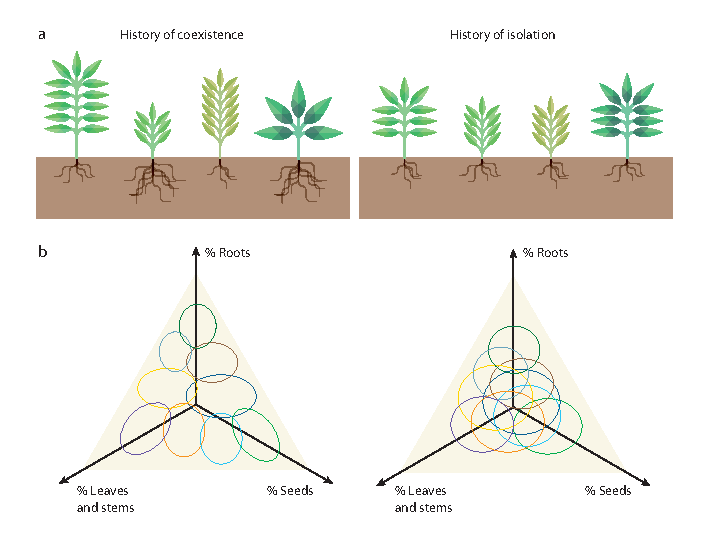
\includegraphics[width=1\linewidth]{./3_Synthesis/graphics/niche_shift.pdf}%
}{
  \caption[ Evolutionary niche shifts.]{ Evolutionary niche shifts. a) \cite{zuppinger-dingley_selection_2014} find that, when plant species are grown in a common environment, those that have a history of selection in diverse communities develop greater differences in traits than species that have a history of isolation. b) This idea feeds into our understanding of how evolutionary history influences the ecological interactions of species that compete for growth factors such as soil nutrients, light and space. All species face trade-offs. For instance, biomass that is allocated to obtaining soil nutrients (roots) cannot be used to obtain light (leaves and stems) or to disperse to open sites (seeds). Graphically depicted, the resulting ‘trade-off surface’ (triangles) represents all possible ways in which plant species (ellipses) can allocate their biomass. A history of selection in diverse communities results in greater interspecific differences (less overlap of
ellipses) and more specialization (smaller ellipses) than a history of isolation. From \cite{tilman_diversity_2014}, reproduced with the permission of Springer, license number: 	
4386020602501.}
  \label{fig:niche_shift}
 }
\end{figure*}

The epigenetic changes, that link the experience of the external conditions with species strategies and transmits this information to following generations may play an important role in the character displacement observed in empirical experiments \parencite{zuppinger-dingley_selection_2014}. The ability of coexisting species to express contrasted phenotypes increasing the biodiversity may rely on the phenotypic plasticity\parencite{roscher_contrasting_2015}, but epignetic processes may play a role in the stability of this mechanisms and a long-time effect on biodiversity \parencite{tilman_density_2014}.



% heritaibility and effects

% link with molecular level mechanisms nicotra and 
%
%The previously mentioned concept of an individual experience competing with a 
%Plasticity as a strategy: genetic dyn + extend the discussion of the limits
%
%heritability: how can it be transfert, wht should be transferred, effect of this heritability (dewiit and barabas)

\paragraph{It is about information}

The development of implementations of the phenotypic plasticity as those listed above introduces a lot of complexity and computational costs. Another approach, at the conceptual end of the modelling approaches, is to consider the external resources and stresses as information to solve an investment problem. Once the gains and cost functions established, the reliability of the information, the uncertainty and the risks can be computed similarly as in other systems such as economic optimisation problems. This would extend the view of the plant physiology as an economic problem \parencite{westoby_time_2000, wright_worldwide_2004, mcmurtrie_leaf-trait_2011}. Such an approach relies on two sides: an explicit and precise description of cost and gain functions, and a prediction of the controlling variables. The former relies on a good understanding of plant physiology, and current knowledges allow a good representation of these processes, but the costs of the plasticity need to be better quantified as already highlighted. The reliability of the information for the prediction of the future conditions has already been pointed out in multiple studies \parencite{dewitt_costs_1998, auld_re-evaluating_2009, richter_phenotypic_2012}. The inability of a plant to consider the cost of being wrong is one argument explaining the low performances observed in \textit{plastic-optimisation} simulations, despite a more flexible plastic allocation resulting in a better exploration of the phenotypic space. The productive, but less efficient phenotypes selected by this algorithm do not authorise errors in the prediction of the resource availability because of their higher sensitivity to unbalanced organ activities. The sensitivity could be considered by evaluating alternative projections of external conditions at the same time as the multiple phenotypes are evaluated. All alternative phenotypes would be evaluated for all probable future conditions. Then an averaging or ranking function would determine the target phenotype from the the best phenotypes under the different projections. While it would increase the computational cost by increasing the dimension of the space explored, better implementation and exploration algorithms could compensate for this downside. In addition, the overall complexity of the model would almost stay the same as it would require only one additional model to weight the chance to optimise the fitness with the risk of unstable phenotypes in case of uncertain prediction.

More advanced learning processes can be investigated to model phenotypic plasticity. The concept of adaptive learning is also a path to explore for the development of the phenotypic plasticity. As genetic algorithms evaluate the success of a strategy by a fitness function at the end of a cycle, individuals could evaluate the performance of plastic response strategies after a few days. The driver of the plasticity resides in the evaluation of the current phenotype for the current and future conditions, in order to eventually develop alternative phenotypes if the performance in not satisfactory\sidenote{this sound finalist, but I use this formulation to emphasise the phenotype evaluation step. This evaluation can take the form of a concentration in a certain stress molecule in a less perspective approach.}. Therefore, in the context of plastic phenotype, the evaluation step quantifies at the same time the success\sidenote{any relevant fitness proxy.} of the current phenotype, but also the success of the plasticity that lead to this phenotype. The plastic strategy is evaluate through the improvement in the phenotype's success, rather than the absolute value of the fitness function. This relative change in fitness must also consider the external stress intensity to avoid penalising well performing plastic strategies under more intense stress. This evaluation of the plasticity strategy allows to adapt the parameters of the plastic response itself, but also the variables required to build the projection of condition, increasing the confidence and reducing the risks of the uncertainty mentioned above. This approach however makes sense under a complex and performing prediction algorithm, and may not fit the scope of the current model that focuses on community dynamics. Specific deigns of plastic plant models will be required to explore this track.

%alternative approach: prediction and the information available

%adaptive learning

%stress also informs on how 


\section{Beyond the simple community}

The previous part of the perspectives that can grow from this work focuses on alternative ways to model phenotypic plasticity or extend the current implementation. But the model already offers a novel tool to explore the effects of phenotypic plasticity on grassland communities dynamics. This aspect has only been scratched and more can easily be done with the current implementation.

\paragraph{The role of the climate}

The first look at the community results highlighted the importance of the fluctuations of the climatic variables. The work presented in the last part can be enriched by a finer analysis of the link between these variables and the properties of the communities. Two points in particular can be investigated: the response to the elevation gradient, and the stability of the productivity. The elevation gradient is of particular interest with the studiy system, as species response may be contrasted  \parencite{kichenin_contrasting_2013}, and plant interaction may evolve \parencite{choler_facilitation_2001, callaway_positive_2002} along this gradient. This last aspect could be investigated in the context of plastic allocation. Indeed, the plasticity may alter these interactions as the results at the community level suggest. This can be investigated with plot simulations or mixed-pot simulation to assess the direct interaction effects. While no clear productivity effect could be observed, the causes of this absence of change has to be identified. Changes in competitive interactions may hide potential effects of plasticity on productivity. In the context of climate change that will certainly increase the amplitude of climatic events \parencite{gobiet_21st_2014}, the stability provided by plasticity in forest ecossytems \parencite{morin_temporal_2014} should also be studied in mountain grasslands.

During this work, weather history as well as climatic projections have been gathered for multiple sites. This information can be used for the gradient analysis proposed above, but also the exploration of climatic scenarios. The combination of these scenarios \parencite{intergovernmental_panel_on_climate_change_climate_2014} with \model offer a powerful tool. Far from being realistic, the model still offers a way to model community dynamics with more temporal and spatial resolution and range than the transplant experiments deployed in empirical studies \parencite{ishizuka_modeling_2012, wang_asymmetric_2014, grassein_importance_2014, hamann_evidence_2016} to simulate the climate change alone, or in combinason with management scenarios \parencite{deleglise_drought-induced_2015}. In particular it gives a way to model the dynamics of competitors \parencite{alexander_novel_2015} with linked communities, but also allows to simulate long-term dynamics and explore many scenarios at low costs.

\paragraph{Calibration and testing}

The available data is not limited to weather data and community composition, as also site specific trait measures are available (from \citet{deleglise_heterogeneite_2011, chalmandrier_communities_2015}). The combination of the site specific weather data with the community specific data should allow a stronger calibration of the global growth parameters. The difficulty to calibrate species specific parameters persists, but taking advantage of both local data, and world wide databases may solve this problem. In particular the estimation of some species specifc morphological parameters should help define ranges for the proportion of active tissues, in agreement with composite traits such as SLA \parencite{john_anatomical_2017} and SRL \parencite{roumet_root_2016}. While some of community level data is available for ungrazed plots, most of the mountain grasslands are exposed to natural and managed grazing. Similarly, frost constitutes a shaping factors of these communities that may be affected by climate change \parencite{choler_growth_2015}. Therefore, it should be accounted and modelled to fully capture the effect of external drivers shapping mountain grasslands. These two drivers, frost hazards and grazing or cutting events are both implemented but should be fully tested to gain realism in the modelled dynamics.

%alexander 2015 - competitors dynamics
%
%take advantage of the already present information,
%build a better calibration -> more precise, prediction
%frei: migration or not ? (phenotlogy) connected sites. asymmetry is sensitivy (more sentive to hotting) wang2014
%
%
%consider the already implemented feature: frost stress and grazing/cutting.
%\paragraph{The climate change}
%
%precise, calibrated model, closer to real systems to link to ES, with proper landscape dyns.
%
%management scenarios and climate scenarios, intreracton \cite{deleglise_drought-induced_2015}

\paragraph{About ecosystem services}

The suggested work on the calibration and testing of the management would allow a better quantification of the communities properties. In addition to allow the assessment of the ecosystem service for these sites \parencite{bello_towards_2010, lavorel_using_2011}, the model could be used to test alternative management practices to optimize service levels \parencite{goslee_optimizing_2013}. The grazing function is simple (pressure and selectivity parameters) but incorporate selective grazing linked to digestibility linked to the plant tissue density \parencite{gardarin_plant_2014}. This functionality coupled with the fine description of the whole community is a handful tool to test scenarios and evaluate service trade-offs to select the best management pathway \parencite{lafond_reconciling_2015}.

Considering multiple services is essential to select optimum management practices to answer broad objectives. Because these service often rely on different properties of the ecosystem \parencite{lavorel_how_2012, lamarque_plant_2014} it is essential to better consider the potential synergies and feedback loops between these properties that were analysed in isolation during this project. Diversity-productivity relationship are often investigated \parencite{tilman_diversity_2001, lepik_high_2005}, but diversity-identity \parencite{zuppinger-dingley_selection_2014} should also be investigated.
%with better calibration, better quantification of measure traits (that were a bit put on the side here) and more specific results (site and weather)
%
%Link the properties together

\paragraph{The meta-community dynamics}

The benefit of having the weather data of multiple sites is also to be able to model explicit meta-community dynamics. While the communities composing the meta-community modelled in the previous were linked only by an infinite artificial seedbank, explicit links can be easily modelled. This seed-bank was necessary to establish the community and stabilise its dynamics. But, once the communities established, the invasion can be limited to the communities modelled rather than an the artificial seed-bank. This allows two things: first, the link between the communities can be explicit and parametrised (\textit{e.g.} the volume of seeds exchanged between two communities can depend on the separating distance), secondly, meta-community-dynamics patterns can emerge from the specific community dynamics and these explicit links. This is interesting in the light of the results at the community levels that show a large impact of the plasticity on the community structure, increasing the species distribution overlap. Also, as mentioned, explicit meta-community dynamics can help us understand the migration/adaptation dynamics that can results from the climate change \parencite{morin_comparing_2009}. Also, such link can help us model the different interactions that can arise from climate change, and how migrating species will compete with established adapting species \parencite{alexander_novel_2015}. The plasticity certainly plays a particular role in these processes and may greatly alter the dynamics by promoting local adaptation \parencite{frei_plant_2014, frei_plastic_2014}, especially if there is an asymmetry in the plastic capacity of the species as a function of there altitude of origin \parencite{gugger_lower_2015, nicotra_adaptive_2015}.
%
%Can have a pretty good role: reinforce or mitigate patterns 
%already possible
%
%landscape dynamics fate-h, island model
%
%invasion and critical transitions


\paragraph{Wrap-up}

\textbf{The long list of extensions to implement, calibrations to run and analysis to conduct that has just been discussed may contrast with the circumscribed perimeter of the work presented in this thesis. However, it shows that this model is a first step in the consideration of the sources of intra-specific variability, here namely the phenotypic plasticity, in the dynamics of the complex systems that are mountain grasslands. This work opens doors for further exploration, in addition to establish clear non trivial effects of plasticity on the properties and structure of the communities. While further work is needed to fully capture the complexity of plastic responses, it seems to me that the most interesting developments lie in the study of the effects of plasticity on larger-scale dynamics. Modelling these dynamics will be interesting to better identify the underlying processes, thanks to the mechanistic nature of the model, but also to predict future trajectories of these systems and optimise management scenarios.}

%fantasised view of the model but this exitment makes us work.

%Further reading, thinking and rambling about what's developped in the papers.
%
%%\section{Plasticity and resistance to climatic events}
%
%%\section{•}
%
%\subsection{Better calibration}
%
%Better implementation rcpp or data table struture, plasticity mech, to allow bayesian and pattern-oriented calibration. A lot of species and a lot of parameters. Difficult exercice. But strategies should be limited by functions and trade-off, just need to calibrate shared (process related) parameters and not species specific (strategic) paramters. This is what allows the modelling of diverse community. 
%
%
%\section{Competition and feedback}
%This document focuses on how the plant are doing with the given resources (arrow in fig in margin). However, a key element in competition and resource dynamics (point that separate Tilman appraoches from Chesson) is the impact of plant on resource (fig in margin). Both are fundamental for the understanding on plant interactions, and I argue that understanding the former is necessary to understand the later and have a global view on plant competitive interactions on resources. blablabla competition experiments, resistance to resource shortening (Tilman) and relative homogeneity of resource (homogeneous in influx, content, starting pool, ... ?). Using the term homogeneous allows to use fixed terms and processes, while to me there is a ambiguity around competition that can be seen as: (1) the impact on growth, (2) the winner out of a competitive scenario (with resource shortening). In this later case, the approach of part 4 (?) has limited interpretation since they are not competing. We can intuiitively imagine (from our understanding of model's functioning) that  there is a hierarchical effect on growth, but that is probably reversed in case of (1) shared resource pool (big plant may have access to bigger resource pool in open environment), (2) sufficiently quick resource shortening to lead to death events.\\
%
%in margin: figure resource and interaction.\\
%figure competition decomposition of fitness (growth and survival), and growth related to resource pool (try to have graph approach).
%
%competition change vegetation response to climate change \parencite{van_loon_how_2014}
%
%transitivity and competition \cite{levine_beyond_2017} Could it emerge from the current implementation of \model ? Is it stable with plasticity ?
%
%
%\section{Extend to climate change effects}
%
%How plasticity actually affect the effects of climate change: mitigate or amplify, risk of critical transition.
%
%drought resistance experiments to be done.
%
%Higher diversity: higher risk of invasion?
%
%Take advantage of simulated scenarios of climate change.
%
%\section{Going forward: epigenetic and heritability}
%
%fundamental knwowledge 
%
%effect of heritability and genetic effects (evolutionary perspective) Bring the two perspective together. \cite{scheiner_genetics_1989}
%
%Bayesian model of dev. \cite{stamps_bayesian_2016} Talked about the difficulty to match reaction norms with systemic plasticity: evolutionay bayesian approach to species specific reaction norms.
%
%Epigenetic variation creates potential for evolution of plant phenotypic plasticity \cite{zhang_epigenetic_2013}
%See also \cite{dewitt_expanding_2016} for higher moment of reaction norms controlled by genes